\documentclass[a4paper]{article}

\usepackage{inputenc}
\usepackage[british,UKenglish]{babel}
\usepackage{amsmath}
%\usepackage{titlesec}
\usepackage{color}
\usepackage{graphicx}
\usepackage{fancyref}
\usepackage{hyperref}
\usepackage{float}
\usepackage{scrextend}
\usepackage{setspace}
\usepackage{xargs}
\usepackage{multicol}
\usepackage{nameref}

\usepackage{sectsty}
\usepackage{multicol}
\usepackage{multirow}
\usepackage[procnames]{listings}
\usepackage{appendix}

\newcommand\tab[1][1cm]{\hspace*{#1}}
\hypersetup{colorlinks=true, linkcolor=black}
\interfootnotelinepenalty=10000

\newcommand{\cleancode}[1]{\begin{addmargin}[3em]{3em}\texttt{\textcolor{cleanOrange}{#1}}\end{addmargin}}
\newcommand{\cleanstyle}[1]{\text{\textcolor{cleanOrange}{\texttt{#1}}}}


\usepackage[colorinlistoftodos,prependcaption,textsize=footnotesize]{todonotes}
\newcommandx{\commred}[2][1=]{\textcolor{Red}
{\todo[linecolor=red,backgroundcolor=red!25,bordercolor=red,#1]{#2}}}
\newcommandx{\commblue}[2][1=]{\textcolor{Blue}
{\todo[linecolor=blue,backgroundcolor=blue!25,bordercolor=blue,#1]{#2}}}
\newcommandx{\commgreen}[2][1=]{\textcolor{OliveGreen}{\todo[linecolor=OliveGreen,backgroundcolor=OliveGreen!25,bordercolor=OliveGreen,#1]{#2}}}
\newcommandx{\commpurp}[2][1=]{\textcolor{Plum}{\todo[linecolor=Plum,backgroundcolor=Plum!25,bordercolor=Plum,#1]{#2}}}

\def\code#1{{\tt #1}}

\def\note#1{\noindent{\bf [Note: #1]}}

\makeatletter
%% The "\@seccntformat" command is an auxiliary command
%% (see pp. 26f. of 'The LaTeX Companion,' 2nd. ed.)
\def\@seccntformat#1{\@ifundefined{#1@cntformat}%
   {\csname the#1\endcsname\quad}  % default
   {\csname #1@cntformat\endcsname}% enable individual control
}
\let\oldappendix\appendix %% save current definition of \appendix
\renewcommand\appendix{%
    \oldappendix
    \newcommand{\section@cntformat}{\appendixname~\thesection\quad}
}
\makeatother


% "define" Scala
\usepackage[T1]{fontenc}  
\usepackage[scaled=0.82]{beramono}  
\usepackage{microtype} 

\sbox0{\small\ttfamily A}
\edef\mybasewidth{\the\wd0 }

\lstdefinelanguage{scala}{
  morekeywords={abstract,case,catch,class,def,%
    do,else,extends,false,final,finally,%
    for,if,implicit,import,match,mixin,%
    new,null,object,override,package,%
    private,protected,requires,return,sealed,%
    super,this,throw,trait,true,try,%
    type,val,var,while,with,yield},
  sensitive=true,
  morecomment=[l]{//},
  morecomment=[n]{/*}{*/},
  morestring=[b]",
  morestring=[b]',
  morestring=[b]"""
}

\usepackage{color}
\definecolor{dkgreen}{rgb}{0,0.6,0}
\definecolor{gray}{rgb}{0.5,0.5,0.5}
\definecolor{mauve}{rgb}{0.58,0,0.82}

% Default settings for code listings
\lstset{frame=tb,
  language=scala,
  aboveskip=3mm,
  belowskip=3mm,
  showstringspaces=false,
  columns=fixed, % basewidth=\mybasewidth,
  basicstyle={\small\ttfamily},
  numbers=none,
  numberstyle=\footnotesize\color{gray},
  % identifierstyle=\color{red},
  keywordstyle=\color{blue},
  commentstyle=\color{dkgreen},
  stringstyle=\color{mauve},
  frame=single,
  breaklines=true,
  breakatwhitespace=true,
  procnamekeys={def, val, var, class, trait, object, extends},
  procnamestyle=\ttfamily\color{red},
  tabsize=2
}

\lstnewenvironment{scala}[1][]
{\lstset{language=scala,#1}}
{}
\lstnewenvironment{cpp}[1][]
{\lstset{language=C++,#1}}
{}
\lstnewenvironment{bash}[1][]
{\lstset{language=bash,#1}}
{}
\lstnewenvironment{verilog}[1][]
{\lstset{language=verilog,#1}}
{}



%代码段设置
\lstset{numbers=left,
basicstyle=\tiny,
numberstyle=\tiny,
keywordstyle=\color{blue!70},
commentstyle=\color{red!50!green!50!blue!50},
frame=single, rulesepcolor=\color{red!20!green!20!blue!20},
escapeinside=``
}

\graphicspath{ {images/} }
\usepackage{ctex}
\usepackage{graphicx}
\usepackage{color,framed}%文本框
\usepackage{listings}
\usepackage{caption}
\usepackage{amssymb}
\usepackage{enumerate}
\usepackage{xcolor}
\usepackage{bm} 
\usepackage{lastpage}%获得总页数
\usepackage{fancyhdr}
\usepackage{tabularx}  
\usepackage{geometry}
\usepackage{minted}
\usepackage{graphics}
\usepackage{subfigure}
\usepackage{float}
\usepackage{pdfpages}
\usepackage{pgfplots}
\pgfplotsset{width=10cm,compat=1.9}
\usepackage{multirow}
\usepackage{footnote}
\usepackage{booktabs}

%-----------------------伪代码------------------
\usepackage{algorithm}  
\usepackage{algorithmicx}  
\usepackage{algpseudocode}  
\floatname{algorithm}{Algorithm}  
\renewcommand{\algorithmicrequire}{\textbf{Input:}}  
\renewcommand{\algorithmicensure}{\textbf{Output:}} 
\usepackage{lipsum}  
\makeatletter
\newenvironment{breakablealgorithm}
  {% \begin{breakablealgorithm}
  \begin{center}
     \refstepcounter{algorithm}% New algorithm
     \hrule height.8pt depth0pt \kern2pt% \@fs@pre for \@fs@ruled
     \renewcommand{\caption}[2][\relax]{% Make a new \caption
      {\raggedright\textbf{\ALG@name~\thealgorithm} ##2\par}%
      \ifx\relax##1\relax % #1 is \relax
         \addcontentsline{loa}{algorithm}{\protect\numberline{\thealgorithm}##2}%
      \else % #1 is not \relax
         \addcontentsline{loa}{algorithm}{\protect\numberline{\thealgorithm}##1}%
      \fi
      \kern2pt\hrule\kern2pt
     }
  }{% \end{breakablealgorithm}
     \kern2pt\hrule\relax% \@fs@post for \@fs@ruled
  \end{center}
  }
\makeatother
%------------------------代码-------------------
\usepackage{xcolor} 
\usepackage{listings} 
\lstset{ 
breaklines,%自动换行
basicstyle=\small,
escapeinside=``,
keywordstyle=\color{ blue!70} \bfseries,
commentstyle=\color{red!50!green!50!blue!50},% 
stringstyle=\ttfamily,% 
extendedchars=false,% 
linewidth=\textwidth,% 
numbers=left,% 
numberstyle=\tiny \color{blue!50},% 
frame=trbl% 
rulesepcolor= \color{ red!20!green!20!blue!20} 
}

%-------------------------页面边距--------------
\geometry{a4paper,left=2.3cm,right=2.3cm,top=2.7cm,bottom=2.7cm}
%-------------------------页眉页脚--------------
\usepackage{fancyhdr}
\pagestyle{fancy}
\lhead{\kaishu \leftmark}
% \chead{}
\rhead{\kaishu 并行程序设计实验报告}%加粗\bfseries 
\lfoot{}
\cfoot{\thepage}
\rfoot{}
\renewcommand{\headrulewidth}{0.1pt}  
\renewcommand{\footrulewidth}{0pt}%去掉横线
\newcommand{\HRule}{\rule{\linewidth}{0.5mm}}%标题横线
\newcommand{\HRulegrossa}{\rule{\linewidth}{1.2mm}}
\setlength{\textfloatsep}{10mm}%设置图片的前后间距
%--------------------文档内容--------------------

\begin{document}
\renewcommand{\contentsname}{目\ 录}
\renewcommand{\appendixname}{附录}
\renewcommand{\appendixpagename}{附录}
\renewcommand{\refname}{参考文献} 
\renewcommand{\figurename}{图}
\renewcommand{\tablename}{表}
\renewcommand{\today}{\number\year 年 \number\month 月 \number\day 日}

%-------------------------封面----------------
\begin{titlepage}
    \begin{center}
    
\includegraphics[width=0.8\textwidth]{NKU.png}\\[1cm]
    \vspace{20mm}
		\textbf{\huge\textbf{\kaishu{计算机学院}}}\\[0.5cm]
		\textbf{\huge{\kaishu{并行程序设计实验报告}}}\\[2.3cm]
		\textbf{\Huge\textbf{\kaishu{作业二:体系结构及性能相关测试}}}

		\vspace{\fill}
    
    % \textbf{\Large \textbf{并行程序设计期末实验报告}}\\[0.8cm]
    % \HRule \\[0.9cm]
    % \HRule \\[2.0cm]
    \centering
    \textsc{\LARGE \kaishu{姓名\ :\ 张明昆}}\\[0.5cm]
    \textsc{\LARGE \kaishu{学号\ :\ 2211585}}\\[0.5cm]
    \textsc{\LARGE \kaishu{专业\ :\ 计算机科学与技术}}\\[0.5cm]
    
    \vfill
    {\Large 2024年3月22日}
    \end{center}
\end{titlepage}

\newpage
\thispagestyle{empty}
\renewcommand{\abstractname}{\kaishu \sihao \textbf{摘要}}
\renewcommand {\thefigure}{\thesection{}.\arabic{figure}}%图片按章标号
\renewcommand{\figurename}{图}
\renewcommand{\contentsname}{目录}  
\cfoot{\thepage\ of \pageref{LastPage}}%当前页 of 总页数


% 生成目录
\clearpage
\tableofcontents
\newpage

%--------------------------Title--------------------------------
\section{实验目标}
    \begin{enumerate}
      \item 以矩阵每一列与向量的内积为例,通过编写代码实践cache优化算法。
      \item 以求数组累加和为例,通过编写代码实践两路链式相加、循环展开和递归相加等超标量优化算法。
      \item 利用prof和uprof等工具,通过运行计时和事件计数的方法,量化分析普通算法和优化算法之间的性能差异。
    \end{enumerate}
\section{实验环境}
   \subsection{X86平台}
      X86平台使用的是一台笔记本电脑,具体参数如下:
      \begin{minted}[mathescape,
                     linenos,
                     numbersep=5pt,
                     gobble=2,
                     frame=lines,
                     framesep=2mm,
                     highlightcolor=green!40]{bash}
         Architecture:                    x86_64
         CPU(s):                          8
         L1d cache:                       128 KiB
         L1i cache:                       256 KiB
         L2 cache:                        2 MiB
         L3 cache:                        4 MiB
      \end{minted}
  \subsection{ARM平台}
  ARM平台使用课程提供的服务器,具体参数如下:
      \begin{minted}[mathescape,
                     linenos,
                     numbersep=5pt,
                     gobble=2,
                     frame=lines,
                     framesep=2mm,
                     highlightcolor=green!40]{bash}
         Architecture:          aarch64
         CPU(s):                96
         L1d 缓存:          64K
         L1i 缓存:          64K
         L2 缓存:           512K
         L3 缓存:           49152K
      \end{minted}
\section{实验设计及分析}
    \subsection{cache优化}
          \subsubsection{实验设计}
                在针对给定问题的改进算法设计中,需考虑到矩阵在内存中是以行优先顺序存储的事实。这种存储方式意味着内存中矩阵的数据按行连续排列,对于逐列访问的算法,这种存储模式会导致较高的缓存未命中率。具体来说,CPU从内存中预取连续的数据块至缓存时,这些数据块可能仅包含计算特定列元素所需的部分数据。因此,计算下一元素时,CPU可能需要重新从较低层次的缓存或主内存中获取数据,由于访问内存的延迟远高于执行计算的时间,这种访问模式显著降低了程序的执行效率。
                
                为了缓解这一问题,提出采用逐行访问并进行cache优化的算法,旨在最大化利用每次缓存中预取的行数据。算法通过对当前预取到cache中的一整行数据进行计算,并将计算结果累加到结果数组的相应位置,从而减少对主内存的访问频率,优化了数据的缓存利用率。虽然此策略并未直接减少计算量,但通过降低数据访问延迟,有效提高了程序整体的执行效率。
                
                进一步地,为了降低算法执行中的条件判断和指令跳转等开销,对逐行访问算法进行循环展开优化。通过在单次迭代中计算多个元素的值,此方法不仅减少了循环次数,还能够充分利用CPU的多条执行流水线,提升超标量处理器的计算性能。循环展开策略通过减少循环控制逻辑的开销,进一步提高了算法的执行效率,尤其在处理大规模数据时表现显著。
          \subsubsection{实验分析}
              我分别设计了三种算法,分别是原始算法、cache优化算法、和循环展开优化算法。并在x86架构的PC上测量了n<=4096三种算法所消耗的时间,实验测试数据如图\ref{fig:all1}所示,其中,矩阵行列数在实验中以16为步进。
                  \begin{figure}[!htbp]
                    \centering
                    \subfigure[n<400]{
                    \begin{minipage}[t]{0.5\linewidth}
                    \centering
                    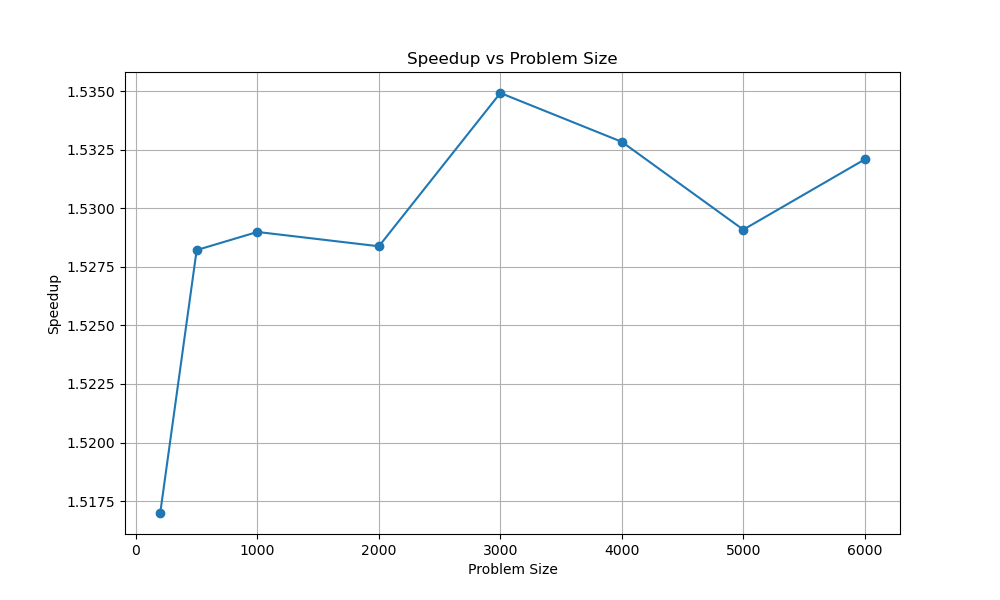
\includegraphics[width=3.2in]{fig/Figure_2.png}
                    \label{fig:mat1}
                    \end{minipage}%
                    }%
                    \subfigure[n<4096]{
                    \begin{minipage}[t]{0.5\linewidth}
                    \centering
                    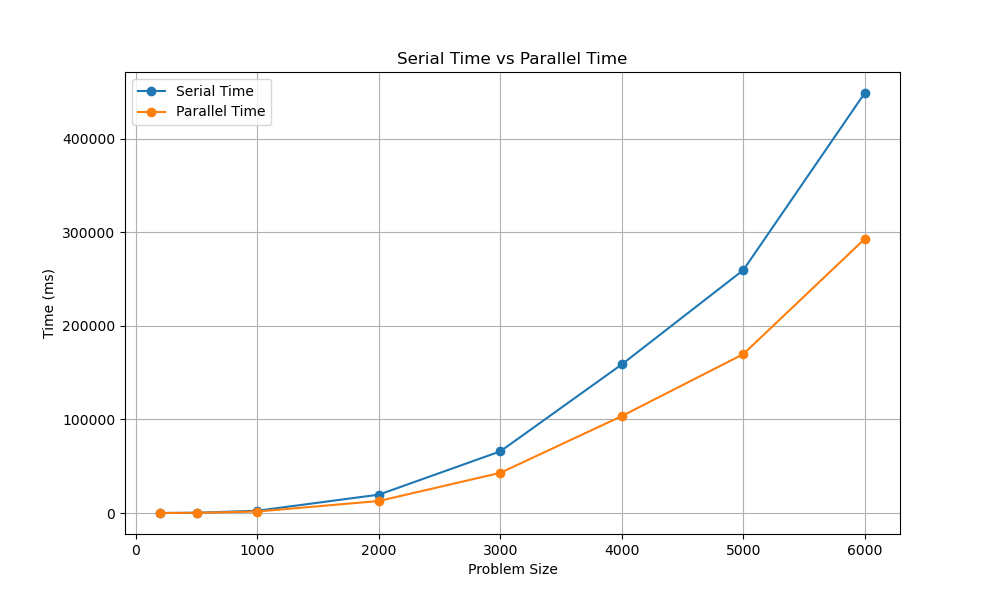
\includegraphics[width=3.2in]{fig/Figure_1.png}
                    \end{minipage}%
                    }
                    \centering
                    \caption{算法消耗时间随问题规模的变化}
                    \label{fig:mat2}
                    \label{fig:all1}
                \end{figure}
                在研究矩阵访问优化方法时,通过对不同数据规模(N)下算法性能的测试分析,我发现在小规模数据(N<300)情况下,如图\ref{fig:mat1}所示,逐行与逐列访问方式的性能差异不显著,我猜测这主要因为CPU缓存(L1和L2)的较快访问速度能够缓解访存延迟的影响。即使L1 cache的命中率已经很低了,但是由于L2 cache的访问速度相对较快,所以访存时间差距不大。然而,引入循环展开技术的优化算法在此情境下即显示出显著的性能提升。
                
                随着数据规模的增加(300<N<3000),逐行访问相比于逐列访问的性能增长速度更慢,时间的差距迅速拉开。表明在这一数据规模下,缓存优化的效果开始显现。猜测这一现象与CPU缓存的层级结构和容量密切相关:L1 cache为64KB,L2为512KB,L3为48MB。由于每个unsigned long long int类型元素占据10字节,可估算出各级cache能容纳的元素数量分别约为80,200,2000。数据规模进一步扩大到N>3000时,逐列访问的效率明显低于逐行访问,因为此时L3 cache的命中率也降低,导致频繁的内存访问,增加了显著的访存开销。
                \begin{table}[h]
                    \centering
                    \caption{不同规模下普通算法和cache优化算法各级cache访问次数和命中情况}
                    \label{tab:cache_performance}
                    \begin{tabular}{|c|c|c|c|c|c|c|}
                    \hline
                    \multicolumn{7}{|c|}{Ordinary} \\
                    \hline
                    n & L1 Hit & L1 Miss & L2 Hit & L2 Miss & L3 Hit & L3 Miss \\
                    \hline
                    80 & 7.81E+07 & 3.19E+05 & 3.11E+05 & 7.91E+03 & 2.64E+02 & 1.20E+01 \\
                    300 & 1.45E+08 & 1.31E+07 & 1.28E+07 & 2.13E+05 & 1.63E+05 & 1.50E+02 \\
                    4000 & 1.49E+08 & 1.58E+07 & 1.19E+07 & 3.93E+06 & 2.39E+06 & 8.89E+05 \\
                    \hline
                    \multicolumn{7}{|c|}{Optimized} \\
                    \hline
                    n & L1 Hit & L1 Miss & L2 Hit & L2 Miss & L3 Hit & L3 Miss \\
                    \hline
                    80 & 9.14E+07 & 4.08E+03 & 3.86E+03 & 1.37E+02 & 1.20E+02 & 0.00E+00 \\
                    300 & 1.83E+08 & 5.62E+04 & 5.11E+04 & 5.12E+03 & 9.36E+02 & 0.00E+00 \\
                    4000 & 1.45E+08 & 8.02E+04 & 7.65E+04 & 3.76E+03 & 3.57E+02 & 8.70E+01 \\
                    \hline
                    \end{tabular}
                \end{table}
                
为了验证上述理论,本研究设计了两组实验,分别在数据规模为64、256和4096的情境下进行,通过利用VTune工具分析其各级缓存的访问频次及命中率,详细数据见表\ref{tab:cache_performance}。

在数据规模为64的实验中,观察到逐列访问相比逐行访问在L1缓存的未命中率显著提高,这导致了对L2缓存的访问次数相应增加。尽管如此,由于L2缓存在大多数情况下都能成功命中,两种访问方式在效率上的差异并不明显。

随着数据规模增至256,逐列访问方式在L2缓存的未命中率明显高于逐行访问,进而导致对L3缓存的访问次数大幅增加。虽然L3缓存的命中率依旧很高,但考虑到访问L3缓存的相对时间成本较高,这一阶段两种方法的性能差距开始显著。

数据规模增至4096时,情况更加明显。逐列访问方式的L3缓存访问次数远超逐行访问,且L3缓存的未命中率高达27.1\%,这意味着需要进行大量的内存访问,因而时间成本极高,这成为了两种方法性能差异巨大的关键所在。
                
                进一步的测试在X86平台上揭示了算法性能在特定数据规模时出现了尖峰现象。
                在n=1024处,算法执行时间出现了一个明显的尖峰,如图\ref{fig:mat3}所示
                除该尖峰外,整个曲线也呈现出有规律的上下波动,经过几次重复实验后,发现曲线上相近的位置仍然存在尖峰。
                  \begin{figure}[!htbp]
                    \centering
                    \subfigure[曲线在n=1024处出现的尖峰]{
                    \begin{minipage}[t]{0.5\linewidth}
                    \centering
                    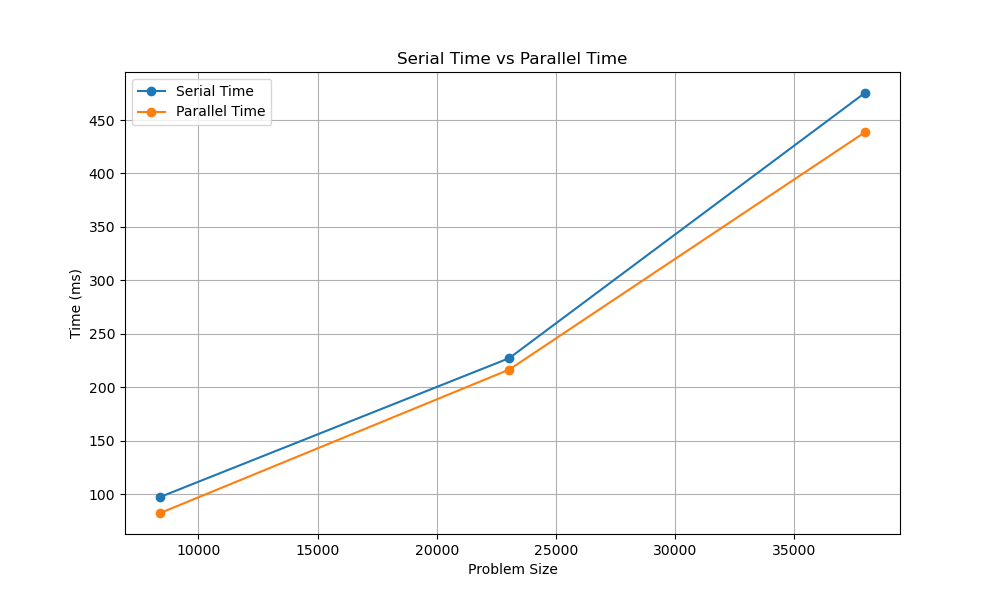
\includegraphics[width=3.2in]{fig/Figure_3.png}
                    \label{fig:mat3}
                    \end{minipage}%
                    }%
                    \subfigure[Cache的结构 - Cache Line]{
                    \begin{minipage}[t]{0.5\linewidth}
                    \centering
                    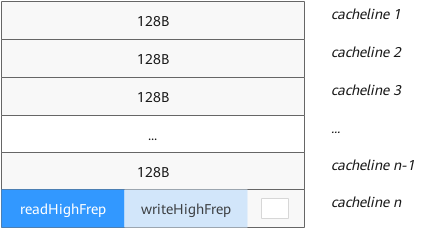
\includegraphics[width=3.2in]{fig/cache_line.png}
                    \end{minipage}%
                    }
                    \centering
                    \caption{}
                    \label{fig:cache_line}
                \end{figure}
                在perf 事件计数测量时发现,当矩阵行数为 1024 时,L1-dcache-load-misses 的事
                件数量比矩阵行数为 1036 时多了 60\%。进一步分析汇编代码,发现这些事件基本都集中在提取矩阵
                mat[j][i] 这个操作上。查阅资料后发现,这个问题可能和 cache 的结构有关,在现代处理器上,
                Cache 划分成了 128 字节的小块,这种小块被称为 Cache Line,而同一个 Cache Line 是不可被同时访
                问的。由于出现尖峰的曲线对应的是列主访问的算法,行列数为整倍数的矩阵导致每次从 Cache 中提
                取元素都需要跨行访问,导致了额外的开销。也有可能由于超标量的特性,可能存在两条指令同时需
                要修改同一个 Cache Line 中的内容的情况,这就造成了伪共享(false sharing)现象,从而导致 Cache
                命中率降低。
    \subsection{超标量优化}
      \subsubsection{实验设计}
对于给定的问题,要求计算 N 个数的和,对于常规的顺序算法而言,由于每次都是在同一个累加
变量上进行累加,导致只能调用 CPU 的一条流水线进行处理,无法充分发挥 CPU 超标量优化的性
能,因此考虑使用多链路的方法对传统的链式累加方法进行改进,即设置多个临时变量,在一个循环
内同时用着多个临时变量对多个不同的位置进行累加,达到多个位置并行累加的效果,同时还能够减
少循环遍历的步长,降低循环开销。由于多链路方法使用了循环展开技术在一定程度上降低了循环的
额外开销,为了保证实验的准确性,我们对普通的链式累加方法也要进行同样比例的循环展开,控制
实验的可变因素,使得实验结果具有合理的对比性。
      \subsubsection{实验分析}
累加实验运行计时的结果如下所示
我测试了从0到70000不同问题规模的算法耗时。如图\ref{fig:all2}所示。

               \begin{figure}[!htbp]
                    \centering
                    \subfigure[x86]{
                    \begin{minipage}[t]{0.5\linewidth}
                    \centering
                    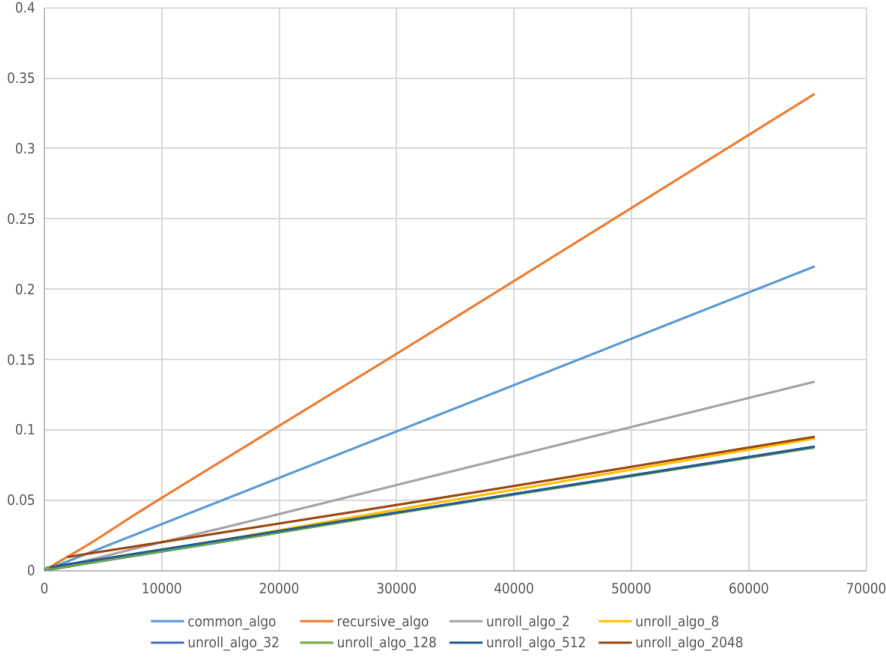
\includegraphics[width=3.2in]{fig/Figure_4.png}
                    \label{fig:sum1}
                    \end{minipage}%
                    }%
                    \subfigure[arm]{
                    \begin{minipage}[t]{0.5\linewidth}
                    \centering
                    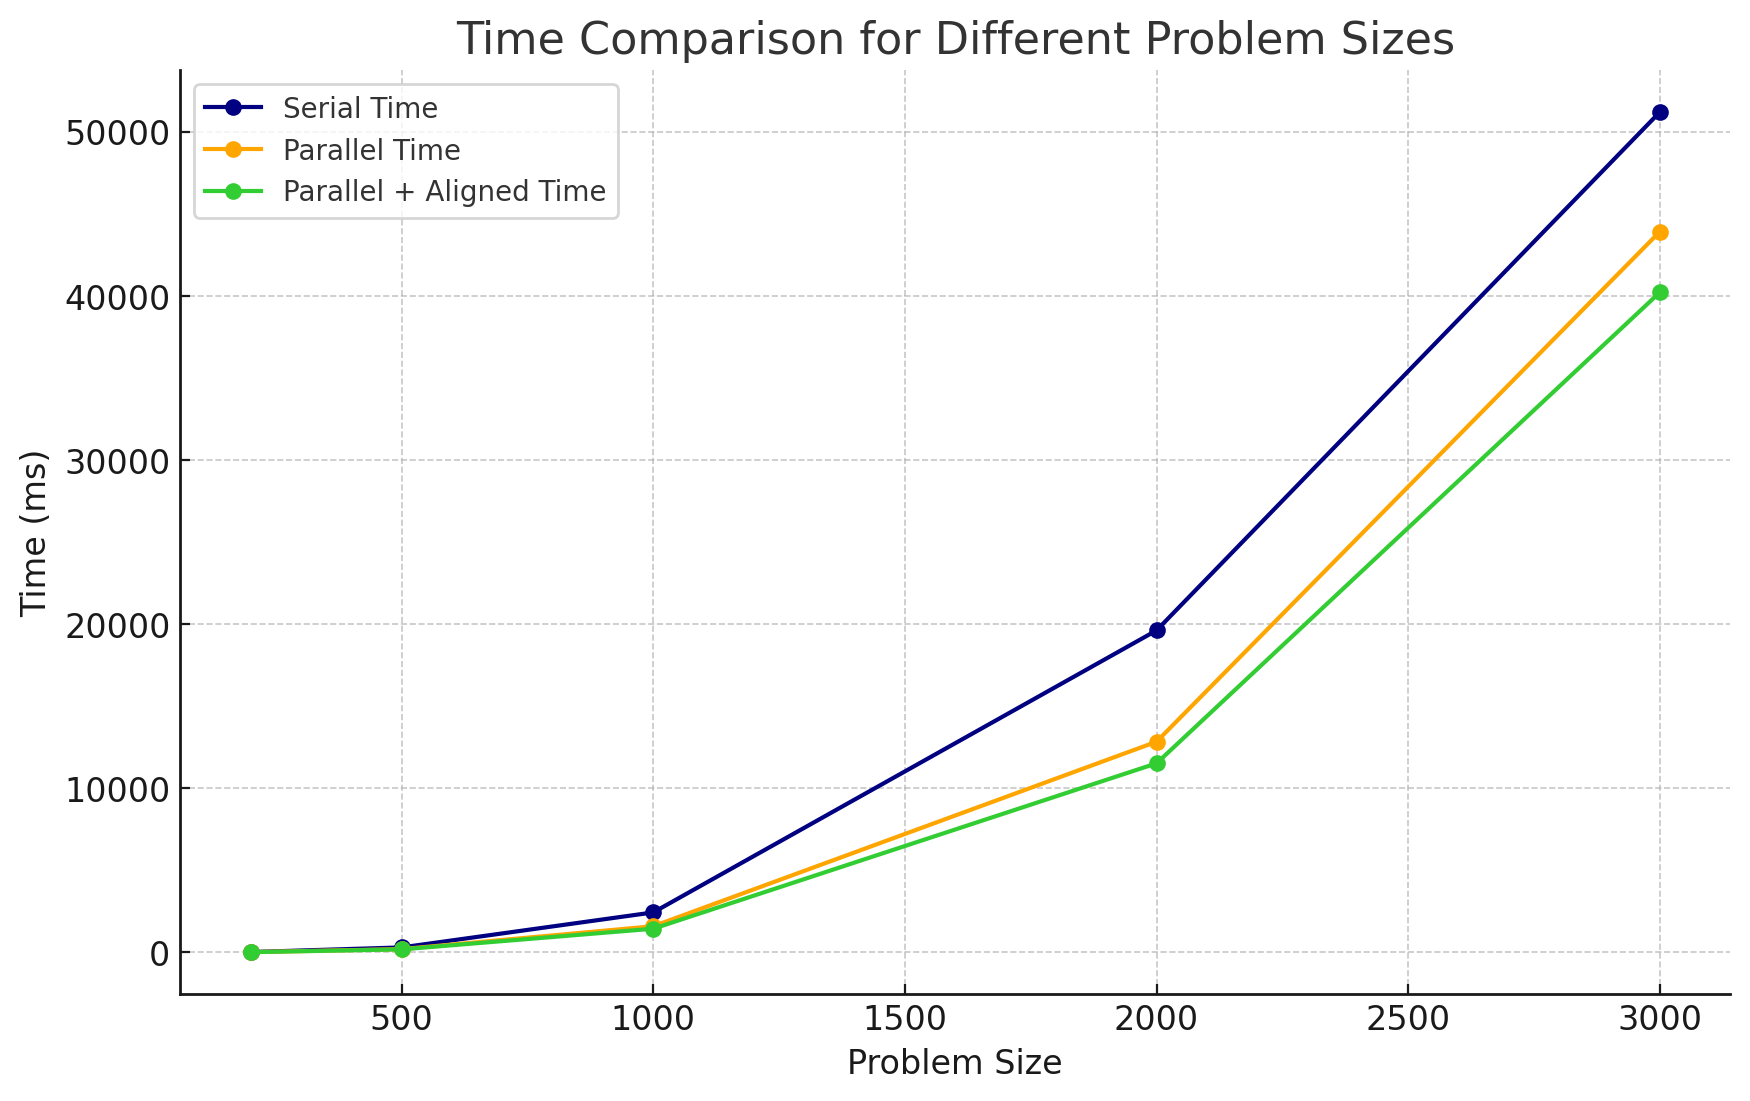
\includegraphics[width=3.2in]{fig/Figure_5.png}
                    \end{minipage}%
                    }
                    \centering
                    \caption{算法消耗时间随问题规模的变化}
                    \label{fig:sum2}
                    \label{fig:all2}
                \end{figure}
从表格数据可见,无论采用链式累加还是多链路展开策略,两者均为线性时间复杂度算法,其执行时间随问题规模增加而成比例增长。然而,采用双链路展开的超标量优化方法在时间效率上明显胜过传统的链式累加策略。原因在于,多链路策略通过解耦相互依赖的累加过程为两个独立的任务,允许CPU同时利用双重流水线进行处理,从而实现了超标量优化。

进一步的证据来自于对比链式累加与多链路累加方法的CPI(每周期指令数)表现。如表\ref{tab:cpi1}所示,多链路累加方法的CPI显著低于链式累加,意味着在相同的时钟周期内,多链路累加能够完成更多的指令处理。这不仅佐证了超标量优化的有效性,也表明我们成功地利用了CPU的多条流水线来提高处理效率
                    \begin{table}[htbp]
                    \centering
                    \caption{普通算法和优化算法的CPI对比}
                    \label{tab:cpi1}
                    \begin{tabular}{@{}lcc@{}}
                    \toprule
                     & 普通算法  & 2路优化算法 \\ \midrule
                    CPI & 0.4975 & 0.4761 \\ \bottomrule
                    \end{tabular}
                    \end{table}
                    

在进行矩阵列向量点积实验时,我注意到ARM平台与X86平台在缓存效率上的表现差异显著,其中ARM平台的整体缓存命中率远高于X86平台(99.158\%相比于96.659\%)。这一现象可能源于ARM平台拥有更为高效的缓存访问机制,并且ARM平台的L1缓存容量更大(64KB对比32KB),从而提高了数据处理的效率。

另一方面,比较两个平台在执行累加操作实验时的运行时间,ARM平台相较于X86平台要长得多,这一差异很可能归因于两者在指令集架构上的根本差异。这表明,虽然ARM平台在缓存效率方面表现出色,但其在某些计算任务上的性能可能受到指令集架构差异的影响,从而影响总体的运行效率。


在图\ref{fig:all2}中展示的结果出乎意料地显示,递归算法在所有比较的算法中效率最低,这一发现与我们的直觉相悖。深入分析表\ref{table:perf_arm_sum}与表\ref{table:perf_X86_sum}揭示了递归算法产生大量的L1-dcache-load-misses事件,原因可能在于递归算法频繁进行非连续内存访问,导致跨越Cache Line,这是降低缓存命中率的主要原因。此外,递归算法本身相对于平凡算法和多路链式算法更为复杂,引入的额外变量可能也对性能产生不利影响。

同时,图\ref{fig:all2}中的数据也揭示了一个有趣的现象:循环展开的效益并非随着展开路数的增加而线性提升。例如,在ARM平台上,2路循环展开与8192路循环展开的性能相差无几。通过对表\ref{table:perf_arm_sum}与表\ref{table:perf_X86_sum}的分析发现,8192路循环展开导致了大量的L1-dcache-load-misses和L1-icache-load-misses事件,从而影响了算法的性能。循环展开增加的每行代码都可能引发misses事件,这些小额的misses累积起来导致了缓存命中率的下降。此外,当输入数据规模增大到超出L1 Cache容量时,后续的循环展开将造成显著的性能损失。这些发现提示我们,在优化算法时,需要权衡循环展开的程度与算法性能之间的关系,避免过度优化导致的性能反而下降。
      \begin{table}[!htbp]
         \centering
         \begin{tabular}{@{}llllll@{}}
         \toprule
         \begin{tabular}[c]{@{}l@{}}优化方法或\\ 循环展开的层数\end{tabular} & cycles       & instructions & CPI    & \begin{tabular}[c]{@{}l@{}}L1-dcache-\\ load-misses\end{tabular} & \begin{tabular}[c]{@{}l@{}}L1-icache-\\ load-misses\end{tabular} \\ \midrule
         不优化                                                     & 13.41\%      & 9.19\%       & 0.6296 & 8.24\%                                                           & 0.00\%                                                           \\
         递归                                                      & 15.55\%      & 18.67\%      & 0.3594 & 15.01\%                                                          & 0.00\%                                                           \\
         2                                                       & 6.73\%       & 7.07\%       & 0.4107 & 6.50\%                                                           & 0.00\%                                                           \\ 
         32                                                      & 4.14\%       & 5.21\%       & 0.3429 & 5.06\%                                                           & 0.00\%                                                           \\
         512                                                     & 4.15\%       & 5.10\%       & 0.3511 & 6.01\%                                                           & 0.00\%                                                           \\
         8192                                                    & 9.89\%       & 6.51\%       & 0.6555 & 8.04\%                                                           & 45.59\%                                                          \\
         事件总数                                                    & 122855688833 & 284706374706 & 0.4315 & 633713953                                                        & 2540277364                                                       \\ \bottomrule
         \end{tabular}
         \caption{ARM平台下累加优化算法的perf事件计数结果}
         \label{table:perf_arm_sum}
         \end{table}
         
         \begin{table}[!htbp]
         \centering
         \begin{tabular}{@{}llllll@{}}
         \toprule
         \begin{tabular}[c]{@{}l@{}}优化方法或\\ 循环展开的层数\end{tabular} & cycles      & instructions & CPI    & \begin{tabular}[c]{@{}l@{}}L1-dcache-\\ load-misses\end{tabular} & \begin{tabular}[c]{@{}l@{}}L1-icache-\\ load-misses\end{tabular} \\ \midrule
         不优化                           & 11.81\%     & 6.92\%       & 0.6762 & 5.70\%                                                           & 2.10\%                                                           \\
         递归                            & 22.60\%     & 17.53\%      & 0.5108 & 16.13\%                                                          & 4.13\%                                                           \\
         2                             & 7.24\%      & 6.70\%       & 0.4281 & 5.51\%                                                           & 1.46\%                                                           \\
         32                            & 4.84\%      & 5.76\%       & 0.3329 & 5.36\%                                                           & 1.30\%                                                           \\
         512                           & 4.64\%      & 5.59\%       & 0.3288 & 5.38\%                                                           & 2.10\%                                                           \\
         8192                          & 5.05\%      & 5.69\%       & 0.3516 & 10.48\%                                                          & 61.37\%                                                          \\
         事件总数                          & 52560137817 & 132651641398 & 0.3962 & 889797839                                                        & 60817536                                                                 \\ \bottomrule
         \end{tabular}
         \caption{X86平台下累加优化算法的perf事件计数结果}
         \label{table:perf_X86_sum}
         \end{table}
\newpage
\section{总结}
在探究给定的矩阵乘法和数组累加问题时,本研究采取了缓存优化和超标量优化策略,旨在提升串行算法的执行效率。通过实验比较,发现对于矩阵乘法问题,逐行访问方式在处理大规模数据集时展现出显著的性能优势。这一优势源于其能够有效提高缓存命中率,由此减少了由内存访问延迟引起的性能损耗。此外,在数组累加实验中,通过引入超标量优化技术——即同时进行多个独立变量的累加操作,以此最终汇总得到总和——能够充分发挥 CPU 多流水线的并行处理能力,从而显著加速程序的执行。这些发现证实了针对特定计算模式采用相应优化策略的有效性。

该实验的全部代码在https://github.com/ftygu/COSC0025-Parallel-Programming-Design中给出。
\end{document}